\documentclass[12pt]{article}
\usepackage[english]{babel}
\usepackage[utf8x]{inputenc}
\usepackage{amsmath}
\usepackage{graphicx}
\usepackage[procnames]{listings}
\usepackage{caption}
\usepackage{parskip} %dannati indent
\usepackage[dvipsnames]{xcolor}
\usepackage{courier}


\lstdefinelanguage{myPython}{
	frameround=fttt,
	frame=trBL,
	tabsize=4, % tab space width
    showstringspaces=false, % don't mark spaces in strings
	numbers=left, % display line numbers on the left
	backgroundcolor=\color{black!10},
	basicstyle=\footnotesize\fontfamily{fvm}\selectfont,
	breaklines=true,
	postbreak=\mbox{\textcolor{red}{$\hookrightarrow$}\space},
	escapeinside={<?}{?>},
	morekeywords = [1]{def, int, float, long, complex, str, unicode, list, tuple, bytearray, buffer},
	keywordstyle = [1]\color{Aquamarine},
	morekeywords = [2]{import,as,return,for,in},
	keywordstyle = [2]\color{OrangeRed},
	morekeywords = [3]{self},
	keywordstyle = [3]\color{orange},
	morekeywords = [4]{=,+,-,>,<,*,.},
	keywordstyle = [4]\color{black},
	alsoletter={<>=-+*},
	procnamekeys={def},
	procnamestyle={\color{YellowGreen}},
}
% \lstset{
% 	keywordstyle=\color{RubineRed}\bfseries, % keyword color
% 	emph={self,null},
% 	emphstyle=\color{Orchid}\bfseries,
% 	backgroundcolor=\color{black!10},
% 	stringstyle=\color{red}, % string color
% }


\begin{document}

\begin{titlepage}

\newcommand{\HRule}{\rule{\linewidth}{0.5mm}} % Defines a new command for the horizontal lines, change thickness here

\center % Center everything on the page
 
%----------------------------------------------------------------------------------------
%	HEADING SECTIONS
%----------------------------------------------------------------------------------------

\textsc{\LARGE Università di Bergamo}\\[1.5cm] % Name of your university/college
\textsc{\Large Relazione progetto}\\[0.5cm] % Major heading such as course name
\textsc{\large Artificial intelligence}\\[0.5cm] % Minor heading such as course title

%----------------------------------------------------------------------------------------
%	TITLE SECTION
%----------------------------------------------------------------------------------------

\HRule \\[0.4cm]
{ \huge \bfseries Reti neurali in python}\\[0.3cm] % Title of your document
\HRule \\[1.5cm]
 
\begin{minipage}{0.4\textwidth}
\begin{flushleft} \large
\emph{Autore:}\\
Dario \textsc{Sardi} % Your name
\end{flushleft}
\end{minipage}
~
\begin{minipage}{0.4\textwidth}
\begin{flushright} \large
\emph{Supervisore:} \\
Francesco \textsc{Trovò} % Supervisor's Name
\end{flushright}
\end{minipage}\\[2cm]
{\large 22 Aprile 2019}\\[2cm] % Date, change the \today to a set date if you want to be precise

\includegraphics[scale=0.5]{logo.png}\\[1cm] % Include a department/university logo - this will require the graphicx package
\vfill % Fill the rest of the page with whitespace

\end{titlepage}
%#######################################################################
\begin{abstract}
L'obiettivo del progetto è quello di creare da zero una rete neurale in python senza sfruttare librerie gia esistenti.
\\Si è creato dapprima un percettrone e successivamente una rete neurale con un solo hidden layer.
\end{abstract}
%#######################################################################
\section{Percettrone}
Per iniziare e prender pratica con eventuali librerie matematiche è stato creato un percettrone, un neurone in grado di compiere semplici scelte binarie.
In quanto classificatore lineare il dataset per il percettrone consiste in una nuvola di punti posizionati randomicamente e pre-classificati in due categorie in base a una funzione lineare stabilita.
\begin{lstlisting}[language=myPython]
def function(x):
	m=-1/3
	c=0.5
	return m*x+c

def genFunction(x,y):
	if y>function(x): return 1
	else: return -1



class point:
    def __init__(self,x,y,b):
		self.pos=[x,y,b]
		self.group=genFunction(x,y)

\end{lstlisting}
In questo modo inizializzando un punto con posizione randomica, la sua appartenenza alle classi \{1,-1\} viene determinata dalla sua posizione relativa alla funzione lineare.
\newpage
\begin{figure}[h!]
	\centering
	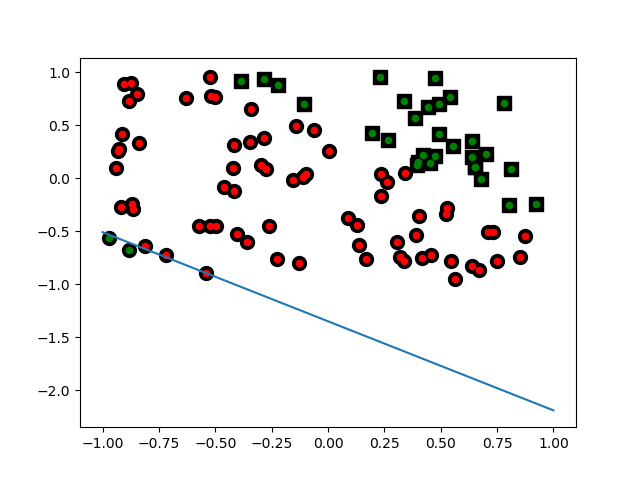
\includegraphics[width=10 cm]{Perc_before.png}
	\caption{classificazione prima del training}
	\label{fig:percBefore}
\end{figure}
Nella rappresentazione grafica (figura \ref{fig:percBefore} ) le due classi son rappresentate con quadrati e cerchi colorati di rosso o verde se sono classificati rispettivamnente in modo corretto o errato.
La funzione effettiva di classificazione è la retta di colore rosso, in blu è presente quella stimata (inizialmente con pesi random).\\
Il programma prosegue con dei cicli di training.
\begin{lstlisting}[language=myPython]
 trainCycle(population, perc, <?\color{magenta}{\textbf{5}}?> )
\end{lstlisting}
Per questo esempio il percettrone viene sottoposto a {\color{magenta}5} cicli di training.
\begin{lstlisting}[language=myPython]
 def <?\color{OliveGreen}{\textbf{TrainCycle}}?>(populationG, pa, number):
	for i in range(number):
		for i in range(50):
			dot = choice(population)
			pa.train(dot.pos, dot.group)
\end{lstlisting}
La funzione {\color{OliveGreen}{\textbf{TrainCycle}}} seleziona 50 elementi randomici (funzione choice in python estrae casualmente da una collezione ) su 100 e li usa come train set.
\newpage
\begin{lstlisting}[language=myPython]
 def train(self,inputs,target):
	guessed = self.guess(inputs)
	error = target-guessed
	for i in range(0,len(self.weights)):
		<?\textcolor{blue}{self.weights[i] += error*inputs[i]*self.lr}?>
\end{lstlisting}
La funzione di train del percettrone rivaluta i propri pesi secondo la formula:

$$\color{blue}\underline{w}=\underline{w}+\underline{err}*\underline{input}*learnRate$$

L'output ottenuto dopo i cicli di training mostra una classificazione corretta.
\begin{figure}[h!]
	\centering
	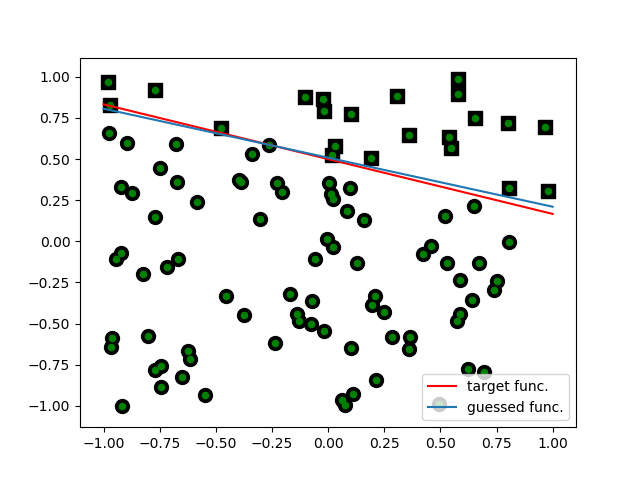
\includegraphics[width=10 cm]{Perc_after.png}
	\caption{classificazione dopo il training}
	\label{fig:percAfter}
\end{figure}
\newpage
%#######################################################################
\section{Doodle classifier}
Lo scopo del progetto è stato ottenere un classificatore in grado di distinguere con una buona precisione a cosa somigliasse di più un disegno rispetto a altri riferimenti passati in precedenza.
\subsection{Neural network}
Il primo passo è stato creare una classe per la rete neurale dotata di un solo hidden layer. 
\begin{lstlisting}[language=myPython]
 def __init__(self, input_size,hidden_size,out_size):
	self.input = []
	self.iS = int(input_size)
	self.oS = int(out_size)

	self.weightsI = np.random.random(( hidden_size,input_size))*2-1
	self.weightsO = np.random.random((out_size,hidden_size))*2-1
	self.bias_h = np.random.random((hidden_size,1))*2-1
	self.bias_o = np.random.random((out_size,1))*2-1
	self.lr = 0.1
	self.output = np.zeros(out_size)
\end{lstlisting}
\begin{figure}[h!]
	\centering
	
\includegraphics[width=10 cm]{resources/hidden.png}
	\caption{rappresentazione matriciale degli argomenti di classe 1}
	\label{fig:hidden}
\end{figure}
\begin{figure}[h!]
	\centering
	
\includegraphics[width=10 cm]{resources/output.png}
	\caption{rappresentazione matriciale degli argomenti di classe 2}
	\label{fig:output}
\end{figure}


\end{document}